% DEVELOPMENT MANUSCRIPT: AI-assisted internal draft for independent verification.
% Not for direct IRIS/ISEF or journal submission.
\documentclass{article}
\usepackage[margin=1in]{geometry}
\usepackage[numbers,sort&compress]{natbib}
\usepackage[utf8]{inputenc}
\usepackage[T1]{fontenc}
\usepackage{graphicx,booktabs,amsmath,hyperref,url}
\usepackage[expansion=false]{microtype}
% Generated from committed result tables by analysis/25_paper_numbers.R.
\newcommand{\OriginalTumorSamples}{541}
\newcommand{\TumorPatients}{533}
\newcommand{\NormalPatients}{72}
\newcommand{\PairedPatients}{72}
\newcommand{\PairedDeg}{8,626}
\newcommand{\PairedCandidatePass}{17}
\newcommand{\MappedDeg}{8,534}
\newcommand{\ReproDeg}{3,323}
\newcommand{\MainSurvival}{1,186}
\newcommand{\SensitivityPass}{1,117}
\newcommand{\StrictGenes}{538}
\newcommand{\HighGenes}{23}
\newcommand{\PriorAdded}{3}
\newcommand{\PriorRemoved}{7}
\newcommand{\AllGeneCount}{32,192}
\newcommand{\AllGeneFdr}{12,630}
\newcommand{\NullOverlapP}{0.178}
\newcommand{\GseMapped}{21}
\newcommand{\GsePatients}{39}
\newcommand{\GseEvents}{17}
\newcommand{\GseSame}{5}
\newcommand{\GseOppositeNominal}{4}
\newcommand{\EmMapped}{22}
\newcommand{\EmPatients}{101}
\newcommand{\EmEvents}{23}
\newcommand{\EmSame}{21}
\newcommand{\EmStrict}{12}
\newcommand{\CompositionFailures}{6}
\newcommand{\BootstrapIntervals}{23}
\newcommand{\ConditionalCvPositive}{23}
\newcommand{\NestedDelta}{0.0039}
\newcommand{\NestedCiLow}{-0.0088}
\newcommand{\NestedCiHigh}{0.0171}
\newcommand{\NestedBrierDelta}{-0.0009}
\newcommand{\NestedClinicalC}{0.744}
\newcommand{\NestedGeneC}{0.747}
\newcommand{\NestedClinicalSlope}{0.86}
\newcommand{\NestedGeneSlope}{0.76}
\newcommand{\NestedDistinctGenes}{10}
\newcommand{\NestedTopGeneFolds}{22}
\newcommand{\NestedNoGeneFolds}{0}
\newcommand{\NestedOutlierFallbacks}{2}
\newcommand{\NestedPassed}{failed}
\newcommand{\NullSelected}{3}
\newcommand{\GseFunnelDelta}{0.042}
\newcommand{\GseFunnelCiLow}{-0.194}
\newcommand{\GseFunnelCiHigh}{0.270}
\newcommand{\GseCompletePresent}{20}
\newcommand{\GseSurvivalPresent}{19}
\newcommand{\EmCompletePresent}{21}
\newcommand{\EmSurvivalPresent}{18}
\newcommand{\FunnelPassed}{failed}
\newcommand{\ShapeNonlinear}{0}
\newcommand{\ShapeTimeVarying}{0}
\newcommand{\TracerxFixedMedian}{98.5}
\newcommand{\TracerxChangingMedian}{86.3}
\newcommand{\TracerxRegions}{186}
\newcommand{\TracerxPatients}{73}
\newcommand{\TracerxEvents}{16}
\newcommand{\TracerxSubsetPatients}{39}
\newcommand{\TracerxSubsetEvents}{9}
\newcommand{\CheckmatePatients}{250}
\newcommand{\CheckmateNivolumab}{120}
\newcommand{\CheckmateEverolimus}{130}
\newcommand{\CheckmateCandidates}{23}
\newcommand{\BenchHydraDelta}{0.0039}
\newcommand{\BenchHydraCiLow}{-0.0081}
\newcommand{\BenchHydraCiHigh}{0.0183}
\newcommand{\BenchHydraSlope}{0.76}
\newcommand{\BenchHydraGenes}{10}
\newcommand{\BenchSurvivalDelta}{-0.0011}
\newcommand{\BenchSurvivalCiLow}{-0.0151}
\newcommand{\BenchSurvivalCiHigh}{0.0139}
\newcommand{\BenchSurvivalGenes}{20}
\newcommand{\BenchDeDelta}{-0.0015}
\newcommand{\BenchDeCiLow}{-0.0120}
\newcommand{\BenchDeCiHigh}{0.0079}
\newcommand{\BenchDeGenes}{5}
\newcommand{\BenchControlDelta}{0.0019}
\newcommand{\BenchControlCiLow}{0.0001}
\newcommand{\BenchControlCiHigh}{0.0039}
\newcommand{\BenchControlGenes}{44}
\newcommand{\BenchRidgeDelta}{0.0257}
\newcommand{\BenchRidgeCiLow}{0.0116}
\newcommand{\BenchRidgeCiHigh}{0.0413}
\newcommand{\BenchRidgeBrier}{-0.0063}
\newcommand{\BenchRidgeBrierCiLow}{-0.0141}
\newcommand{\BenchRidgeBrierCiHigh}{0.0017}
\newcommand{\BenchRidgeSlope}{0.87}
\newcommand{\BenchRidgeGenes}{3,335}
\newcommand{\BenchRidgeGenesMin}{3,067}
\newcommand{\BenchRidgeGenesMax}{3,447}
\newcommand{\BenchClinicalC}{0.744}
\newcommand{\BenchClinicalSlope}{0.86}

\title{Auditing a Transcriptomic Prognostic Funnel in Clear Cell Renal Cell Carcinoma}
\author{HYDRA-ccRCC development manuscript}
\date{}

\begin{document}
\maketitle
\noindent\textbf{Internal development draft. Not for direct submission.}

\begin{abstract}
Tumor--normal differential expression is often treated as a route to prognostic biomarkers, although patient duplication, outcome-dependent selection, tissue composition, and external cohort disagreement can inflate the apparent evidence. We audited HYDRA-ccRCC using one TCGA-KIRC tumor aliquot per patient (\TumorPatients\ tumors and \NormalPatients\ normals), paired expression cohorts, and two previously inspected survival cohorts. The corrected funnel retained \ReproDeg\ reproducible differentially expressed genes, \StrictGenes\ strict candidates, and \HighGenes\ high-confidence candidates, down from 27 in the prior sample-level analysis. The selection-aware ten-repeat, five-fold analysis gave a mean clinical-plus-selected-gene concordance increment of \NestedDelta\ (patient-bootstrap 95\% interval \NestedCiLow\ to \NestedCiHigh) and a three-year Brier-score difference of \NestedBrierDelta; its prespecified criterion \NestedPassed. A matched-list comparison did not establish superiority over survival-only selection (GSE29609 directional-rate difference \GseFunnelDelta; 95\% bootstrap interval \GseFunnelCiLow\ to \GseFunnelCiHigh). E-MTAB-1980 gave strict same-direction support to \EmStrict\ of \EmMapped\ mapped candidates, while GSE29609 retained the TCGA direction for only \GseSame\ of \GseMapped\ and showed FDR-significant reversals for DDC and TCIRG1. No candidate-by-treatment interaction survived FDR correction in the CheckMate 025 RNA subset. These are candidate prognostic associations and audit findings, not a validated biomarker panel.
\end{abstract}

\section{Introduction}
Clear cell renal cell carcinoma (ccRCC) has broad metabolic, vascular, and immune transcriptional changes \cite{tcga_kirc_2013,vhl_hif_review_2024}. A tumor--normal expression difference does not establish independent prognostic value: a signal can arise from the composition of the tissue, and repeated samples from one patient can make survival evidence appear more precise. We audited the public-data HYDRA-ccRCC funnel for these failure modes and tested whether its successive gates outperform simpler gene lists in already inspected external cohorts.

\section{Methods}
\subsection{Inputs, patient identity, and discovery}
TCGA-KIRC STAR unstranded counts and clinical outcomes were retrieved through TCGAbiolinks \cite{colaprico_tcgabiolinks_2016}. For each patient and sample type, we selected the aliquot with greatest raw-count library depth and broke ties by barcode. Survival-event coding was checked against vital status and the appropriate death or follow-up date; joins were required to remain one row per patient. Original retrieval dates for cached public inputs were unavailable, so the repository records source URLs and hashes without assigning new access dates.

DESeq2 compared the selected tumors and normals after requiring at least ten counts in ten samples \cite{love_deseq2_2014}. A separate patient-blocked DESeq2 fit used the \PairedPatients\ selected tumor--normal pairs. GSE40435 and GSE53757 were analyzed with patient-blocked limma; each parsed patient was required to have exactly one tumor and one normal, and surrogate-variable analysis protected the paired contrast \cite{ritchie_limma_2015,leek_sva_2012}. GSE53757 pair IDs were inferred from alternating sample order, so the condition check cannot independently prove patient identity. A reproducible DEG required TCGA FDR below 0.05 and absolute log$_2$ fold change at least one, concordant direction in both GEO cohorts, and nominal support in at least one. A separate apeglm analysis tested all count-QC genes without the fold-change gate; it was not allowed to redefine the primary candidate set \cite{zhu_apeglm_2019}.

The primary Cox model used continuous standardized expression, age, sex, stage, and collapsed grade among complete cases \cite{cox_1972}. The strict gate also required main-model FDR below 0.05, absolute log hazard ratio at least $\log(1.25)$, both GEO effects at least 0.25 in absolute log$_2$ units, and concordant nominal stage-only and grade-only sensitivity fits. The high-confidence gate required FDR below 0.01 and absolute log hazard ratio at least $\log(1.5)$. Proportional-hazards tests were diagnostics, never selection gates.

\subsection{Selection-aware prediction and null simulation}
Ten repeats of five event-stratified patient folds reran TCGA DE and every candidate gate within each training fold. GEO expression evidence remained fixed; test patients and their normals were excluded from training. Library-size normalization and expression scaling were estimated on training samples and applied to held-out tumors. DESeq2 retained the primary outlier-replacement setting, with a logged no-replacement retry only if the pinned runtime failed in that step. The top qualifying gene was added to a clinical Cox model; when no gene qualified, its prediction equaled the clinical-only prediction. Out-of-fold concordance, three-year inverse-probability-of-censoring-weighted Brier score, and calibration slope were computed per repeat. The concordance increment received a patient-resampled 95\% interval. The prespecified success rule required an increment at least 0.01, interval lower limit above zero, and no worse Brier score.

Two hundred clinical-only null datasets used an exponential baseline calibrated to the clinical Cox cumulative hazard with resampled censoring; each reran the full training selection on one held-out fold, cycling across the five fixed folds. This is a null sensitivity under a specific data-generating model, not another ten-by-five-fold interval. The original 1,000 patient bootstraps and 20-repeat per-gene CV condition on the full-data shortlist and remain descriptive rather than selection-adjusted evidence.

\subsection{Exploratory alternatives and biological checks}
At the largest common list size of 22 genes, we compared the complete rule with survival-only, DE-only, each leave-one-GEO-out rule, and TCGA-expression-matched non-prognostic controls. GSE29609 and E-MTAB-1980 were previously inspected, so both evaluations are exploratory. We estimated the complete-rule minus survival-only directional-rate difference and a 2,000-draw paired gene bootstrap in each cohort. The prespecified funnel criterion required an interval entirely above zero.

Candidate Cox models were refit on matched complete cases with published TCGA consensus tumor purity \cite{aran_purity_2015} or leave-one-candidate-out proximal-tubule, endothelial, immune, and stromal marker scores. Nonlinear expression and expression-by-log-time models were tested against the linear proportional-hazards fit. Human Protein Atlas normal-tissue single-cell profiles informed cell-source cautions but were not treated as ccRCC tumor single-cell validation.

TRACERx Renal provided primary-region expression and linked survival data from a pinned public repository \cite{fernandez_sanroman_tracerx_2025}. One thousand repeats selected one region per patient. A fixed event-stratified 39-patient subset isolated region-choice variation; a separate scenario resampled which 39 patients entered each repeat. CheckMate 025 supplementary RNA data supported post hoc continuous-expression-by-treatment Cox interactions for overall and progression-free survival, with FDR correction within endpoint and model \cite{braun_checkmate_2020}.

\section{Results}
\subsection{Corrected discovery and conditional sensitivity}
The original \OriginalTumorSamples\ tumor aliquots represented \TumorPatients\ patients; four patients contributed three aliquots each. Patient-level selection left \NormalPatients\ normals. The paired DE fit included \PairedPatients\ patients and found \PairedDeg\ genes meeting the stated DE threshold. All \HighGenes\ candidates retained their tumor--normal direction, while only \PairedCandidatePass\ met the paired DE threshold; this is a sensitivity to the tumor--normal design, not an independent cohort. The primary analysis found \MappedDeg\ TCGA-significant mapped genes, \ReproDeg\ reproducible DEGs, \MainSurvival\ main-model FDR associations, \SensitivityPass\ sensitivity-pass genes, \StrictGenes\ strict candidates, and \HighGenes\ high-confidence candidates. Relative to the previous 27-gene run, \PriorAdded\ genes entered and \PriorRemoved\ left the shortlist. The all-gene sensitivity modeled \AllGeneCount\ count-QC genes and found \AllGeneFdr\ survival associations at global FDR below 0.05, illustrating how broad the outcome signal becomes without the upstream gate.

\begin{figure}[htbp]
\centering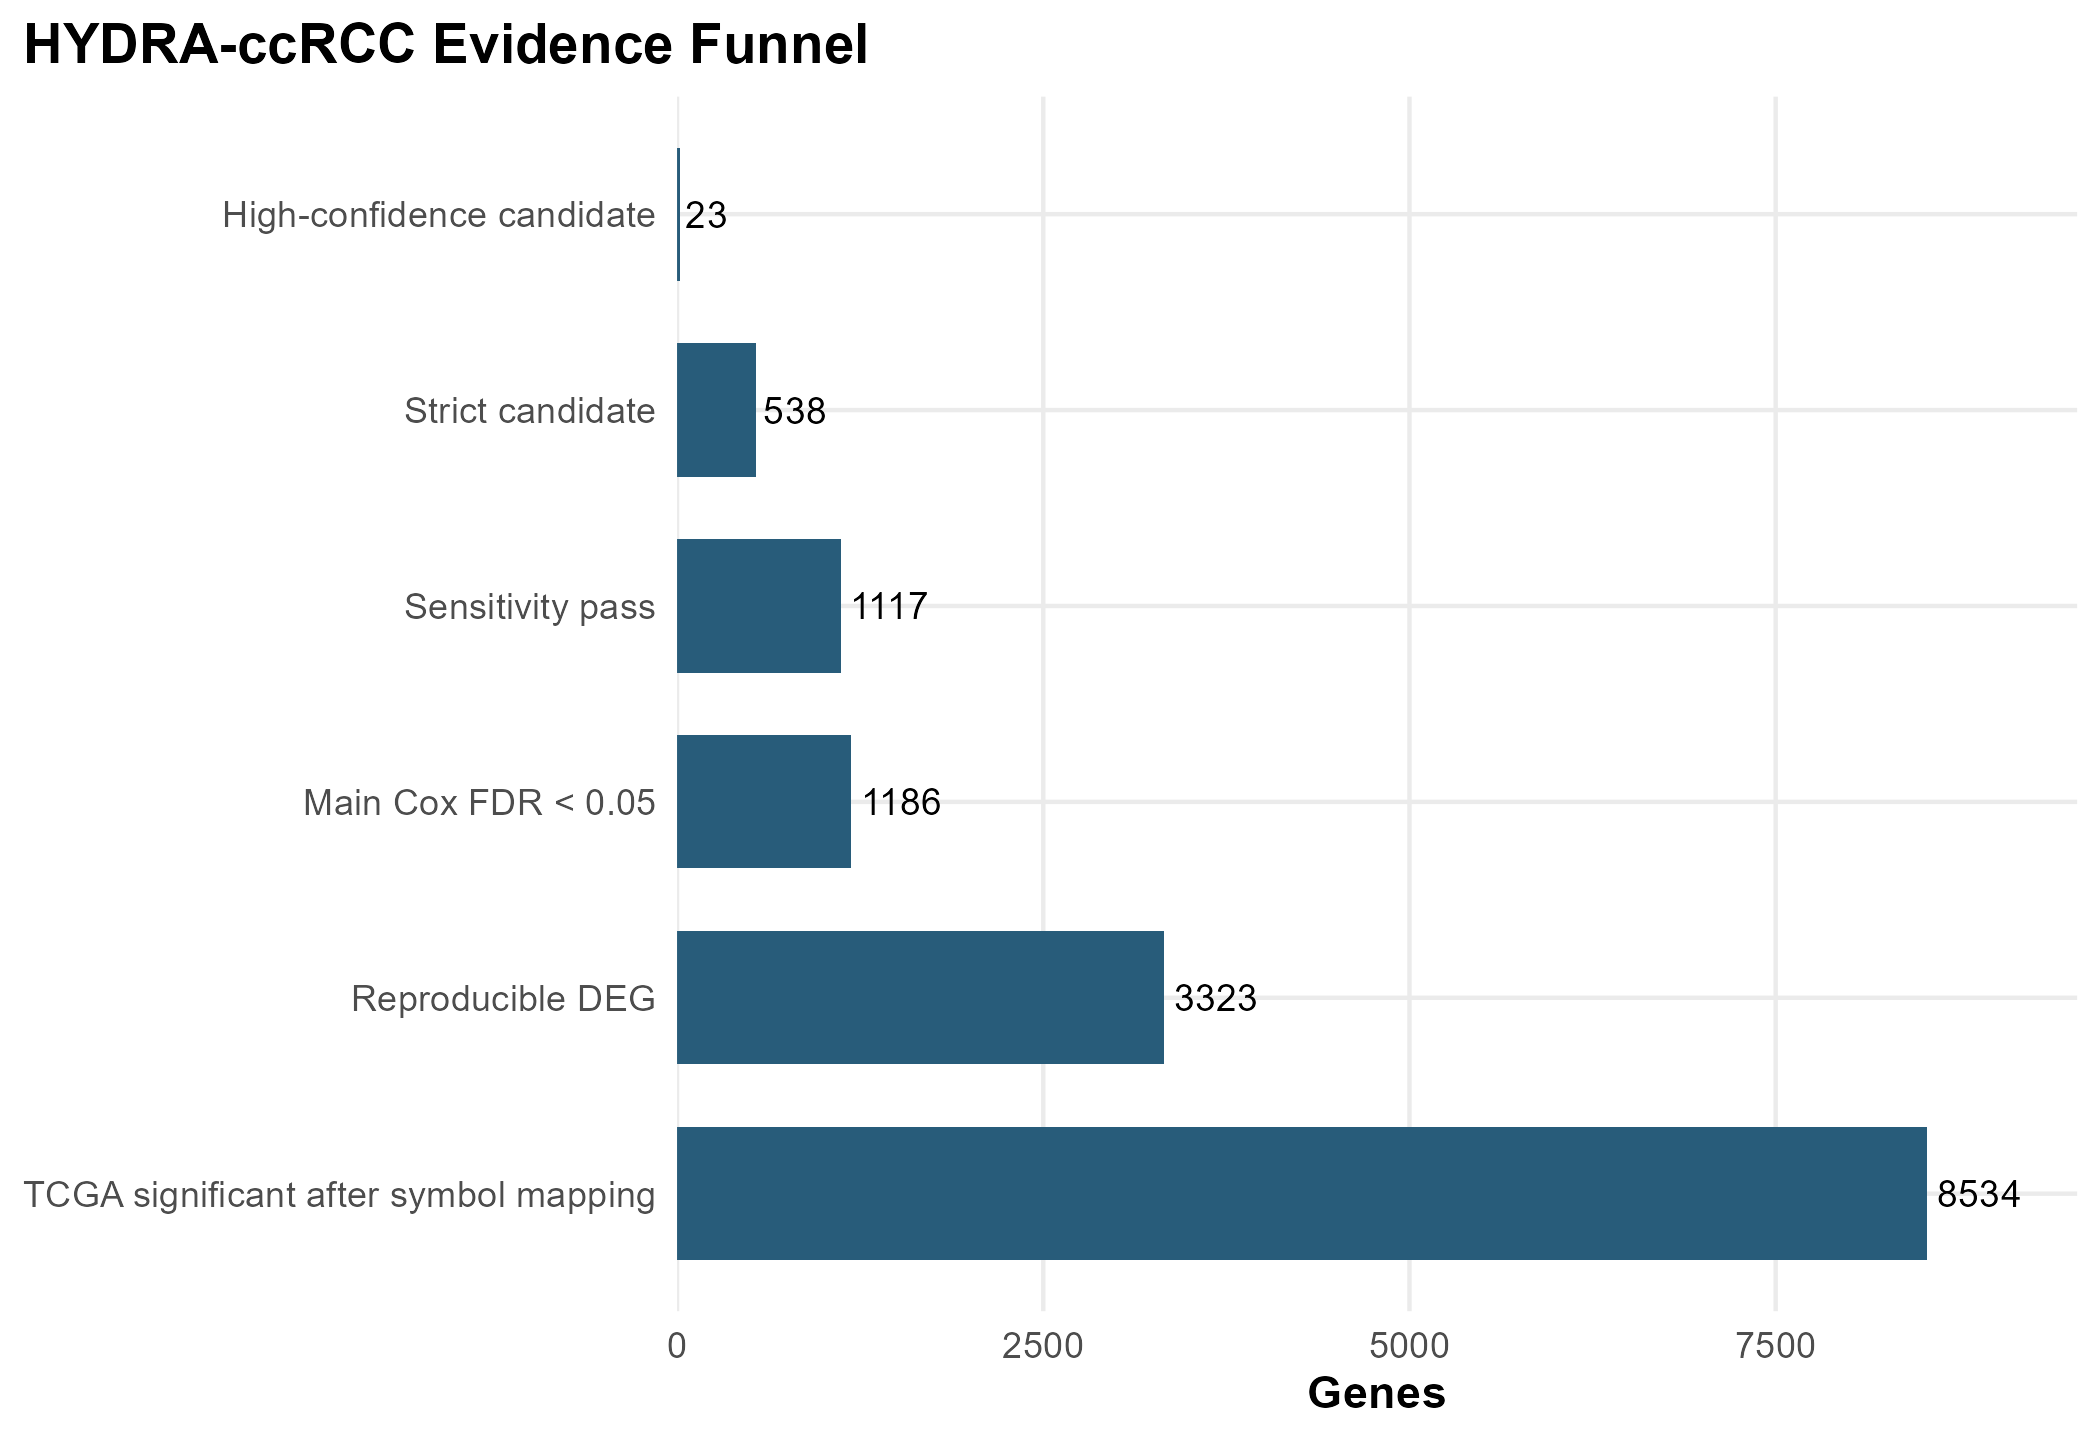
\includegraphics[width=\linewidth]{../results/figures/evidence_funnel.png}
\caption{Corrected patient-level discovery funnel. The candidate set is defined entirely within TCGA and the two GEO expression cohorts.}
\end{figure}

All \HighGenes\ conditional bootstrap intervals excluded zero. The per-gene conditional CV showed positive mean concordance increments for \ConditionalCvPositive\ candidates, but both analyses start from genes chosen on the full TCGA outcome data. They cannot estimate the optimism of the complete selection process.
The within-reproducible-gene overlap permutation did not show enrichment of the GEO-effect gate among survival-pass genes (empirical $p=\NullOverlapP$). It shuffles pass labels rather than refitting survival models, so it is a limited negative control.

\subsection{Selection-aware prediction and funnel comparison}
The nested analysis selected no gene in \NestedNoGeneFolds\ of 50 training folds; \NestedOutlierFallbacks\ folds required a no-replacement retry after a DESeq2 outlier-replacement error. The mean out-of-fold concordance increment was \NestedDelta\ (patient-bootstrap 95\% interval \NestedCiLow\ to \NestedCiHigh); the mean gene-minus-clinical three-year Brier-score difference was \NestedBrierDelta. The predeclared prediction criterion \NestedPassed. The clinical-only null selected a gene in \NullSelected\ of 200 single-fold simulations. These simulations estimate selection under their specified clinical-risk model and do not change the repeated-CV criterion.

\begin{figure}[htbp]
\centering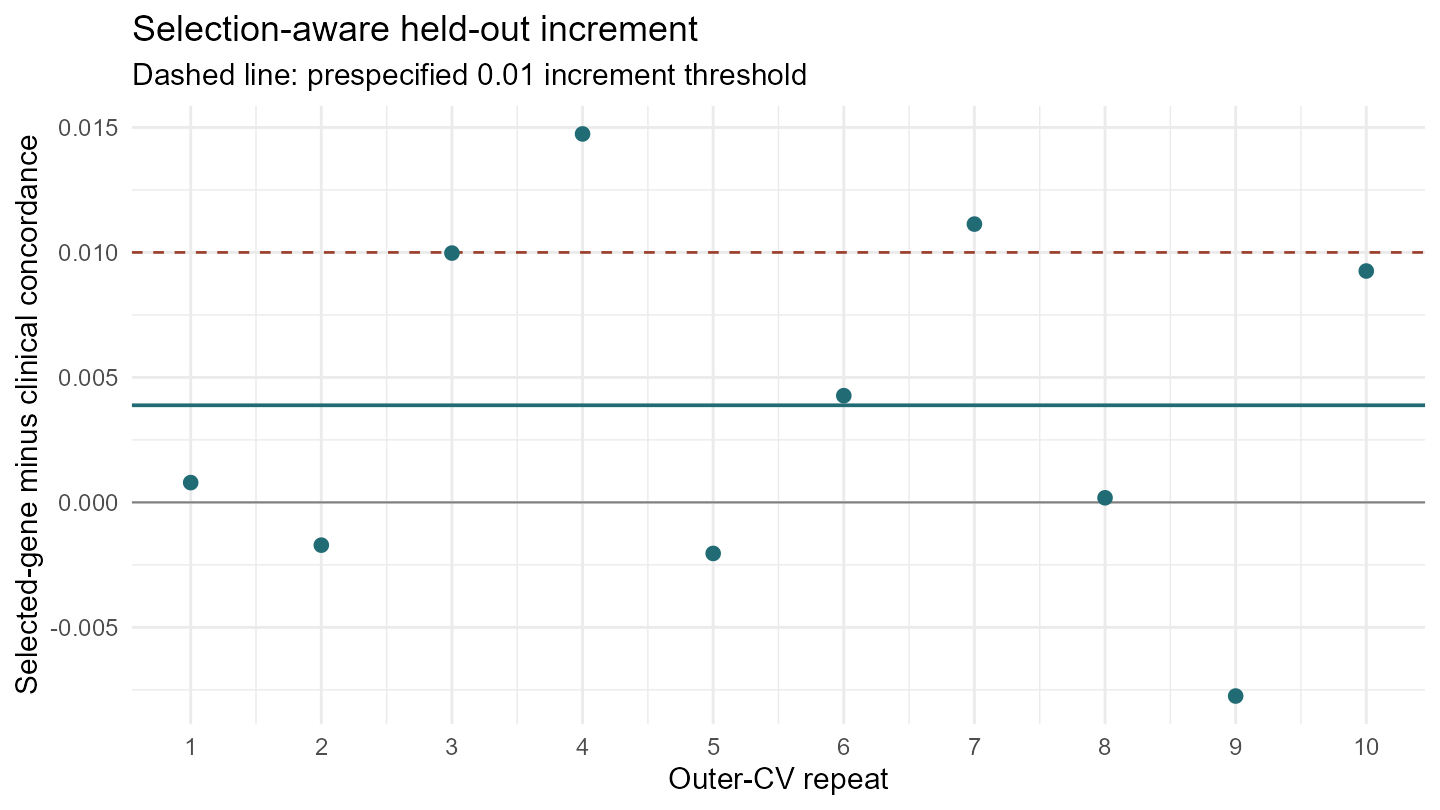
\includegraphics[width=\linewidth]{../results/figures/nested_cv_increment.png}
\caption{Concordance increment across ten complete outer-CV repeats. The dashed line marks the prespecified 0.01 threshold; the patient-bootstrap interval is reported in text.}
\end{figure}

The matched-list funnel criterion \FunnelPassed. In GSE29609 the complete-minus-survival-only directional-rate difference was \GseFunnelDelta\ (paired 95\% interval \GseFunnelCiLow\ to \GseFunnelCiHigh). The E-MTAB-1980 matched lists each had 100\% direction agreement among their mapped genes, so that cohort could not separate the rules on this endpoint. Matching at 22 genes was necessary because one leave-one-GEO-out rule yielded only 22 eligible genes. The comparison reuses already inspected external outcomes and is not confirmatory.

\begin{figure}[htbp]
\centering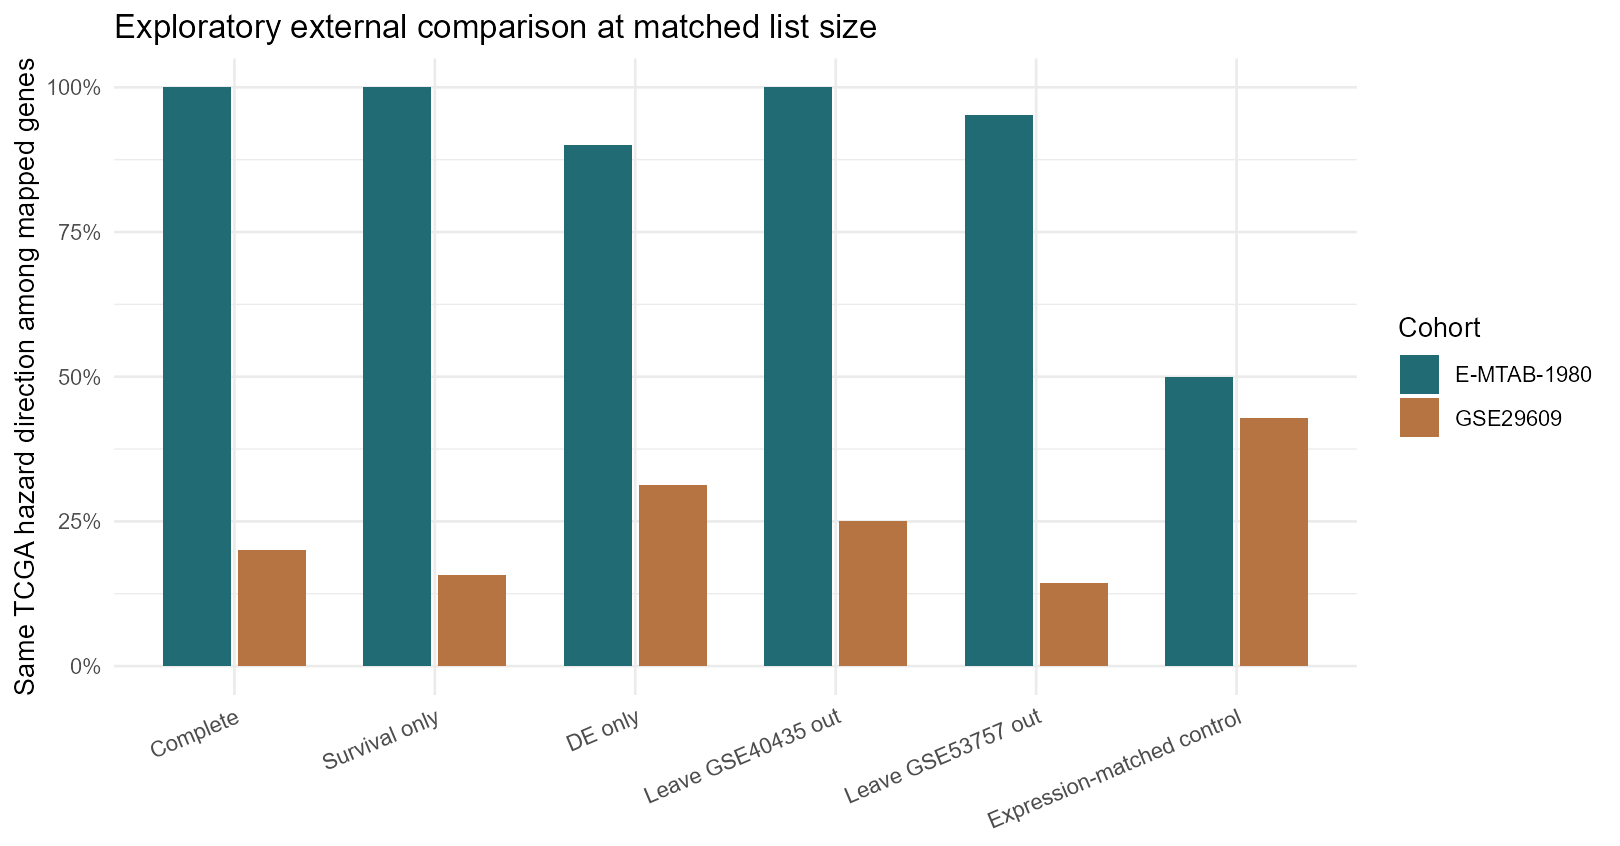
\includegraphics[width=\linewidth]{../results/figures/funnel_external_comparison.png}
\caption{Same-direction replication among mapped genes for six equal-sized lists in two previously inspected cohorts. Different platform coverage and event counts limit comparison.}
\end{figure}

\subsection{External disagreement and composition}
GSE29609 contained \GsePatients\ patients and \GseEvents\ deaths. It mapped \GseMapped\ primary candidates, of which \GseSame\ retained the TCGA hazard direction; \GseOppositeNominal\ had nominal opposite-direction associations. DDC and TCIRG1 were reversed at FDR below 0.05. E-MTAB-1980 contained \EmPatients\ patients and \EmEvents\ deaths, mapped \EmMapped\ candidates, retained the TCGA direction for \EmSame, and gave \EmStrict\ strict same-direction unadjusted and limited-adjustment FDR results. These cohorts disagree sufficiently that the latter cannot be described as universal external replication.

Matched-patient marker-score adjustment removed FDR support for \CompositionFailures\ candidates. Direct consensus-purity adjustment retained direction and FDR support for all \HighGenes\, although consensus purity is inferred rather than a tumor-cell measurement. After correction for 23 tests, \ShapeNonlinear\ nonlinear-expression comparisons and \ShapeTimeVarying\ expression-by-time comparisons had FDR below 0.05. Normal-tissue HPA profiles do not identify ccRCC tumor-cell origin.

\subsection{Spatial sampling and randomized treatment}
TRACERx linked \TracerxRegions\ primary regions from \TracerxPatients\ patients, including \TracerxEvents\ deaths. Across genes, median agreement with the TCGA hazard direction was \TracerxFixedMedian\% when the \TracerxSubsetPatients\ patients were fixed and only the chosen region varied, versus \TracerxChangingMedian\% when both patient membership and region varied. Each smaller subset had \TracerxSubsetEvents\ deaths. Thus, the original small-cohort dispersion conflated two sources of variation and cannot attribute GSE29609's reversals to spatial sampling alone.

The CheckMate 025 RNA subset included \CheckmatePatients\ patients (\CheckmateNivolumab\ nivolumab and \CheckmateEverolimus\ everolimus); all \CheckmateCandidates\ candidates were assessed. No expression-by-treatment interaction survived FDR correction for overall or progression-free survival in either the randomized or limited-adjustment model. Nominal interactions remain exploratory and do not establish treatment selection.

\section{Discussion and limitations}
Correcting patient identity changed the shortlist from 27 to \HighGenes\ genes, yet the more consequential qualification is methodological: conditional coefficient precision and single-gene holdout performance do not answer whether a data-selected funnel predicts new patients. The nested assessment supplies that test, and its prespecified result is reported whether favorable or unfavorable. The matched-list external comparison likewise failed to show a clear advantage over survival-only ranking. Neither result authorizes a deployed multigene panel.

This is a retrospective public-data analysis. GSE29609 has only 17 deaths, E-MTAB-1980 has 23, and both were inspected before this reanalysis; no untouched external patient cohort is available. The 39-patient TRACERx subsets have nine deaths and do not recreate GSE29609's platform or case mix. Consensus purity and bulk marker scores are imperfect composition measures; HPA profiles normal tissue, and tumor single-cell, protein, and functional validation are unavailable. The post hoc CheckMate 025 RNA subset and everolimus comparator do not validate predictive effects in current treatment settings. RNA associations cannot establish a mechanism or therapeutic target.

\section*{Data and reproducibility}
Public source identifiers, the pinned TRACERx commit, cached-input hashes, and package versions are recorded in the repository. The original retrieval dates for cached inputs are unknown. Core result counts and estimates are generated from result tables by \texttt{analysis/25\_paper\_numbers.R} into \texttt{paper/results\_macros.tex}; the pipeline and PDF build are separate reproducible commands. This manuscript is an internal AI-assisted development draft for independent verification before submission.

\section*{Ethics, funding, and AI assistance}
This secondary analysis used public de-identified data and involved no new recruitment or intervention. No external funding was reported. OpenAI Codex assisted with the audit, code, and development manuscript; the student researcher must independently verify every statistical, scientific, and citation claim before any submission.

\section*{Acknowledgments}
The previous development draft thanked Levi Waldron, Michael Love, Philip Saylor, Samra Turajli\'c, and David McDermott for feedback that shaped the analysis. The author remains responsible for the implementation and interpretation; these acknowledgments require author verification before submission.

\bibliographystyle{plainnat}
\bibliography{references}
\end{document}
